\documentclass{standalone}
\usepackage{tikz}
\usetikzlibrary{patterns, positioning}


\begin{document}
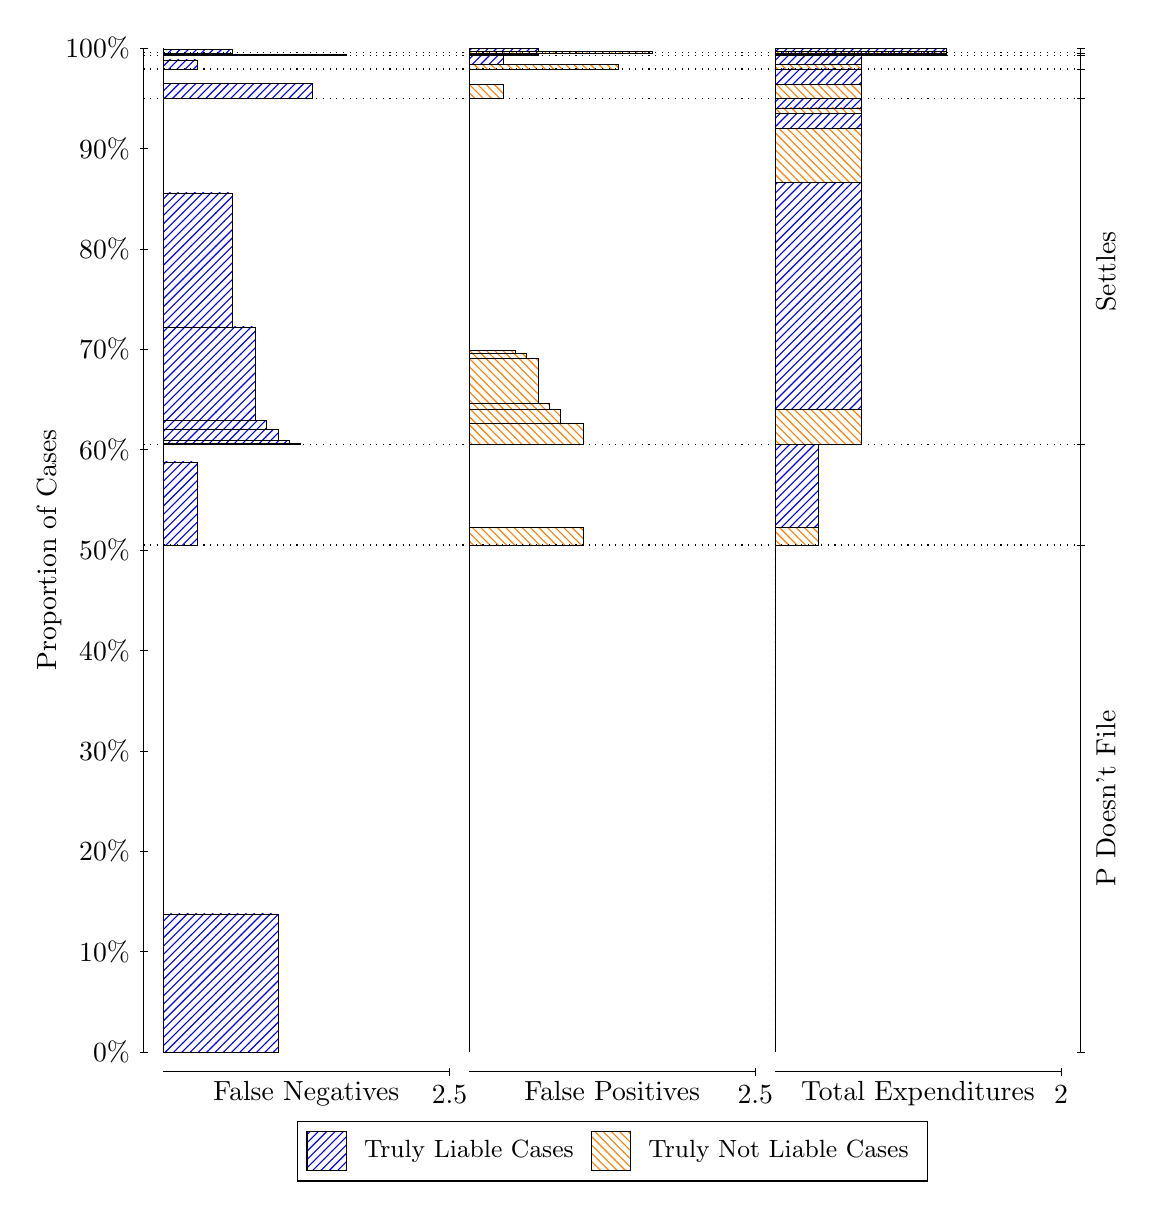
\begin{tikzpicture}
\draw[black, very thin] (1.5,1.75) -- (1.5,14.5);
\node[rotate=90, text=black, anchor=center] at (0.3, 8.125) {Proportion of Cases};
\draw[black, very thin] (1.45,1.75) -- (1.55,1.75);
\node[text=black, anchor=east] at (1.45, 1.75) {0\%};
\draw[black, very thin] (1.45,3.025) -- (1.55,3.025);
\node[text=black, anchor=east] at (1.45, 3.025) {10\%};
\draw[black, very thin] (1.45,4.3) -- (1.55,4.3);
\node[text=black, anchor=east] at (1.45, 4.3) {20\%};
\draw[black, very thin] (1.45,5.575) -- (1.55,5.575);
\node[text=black, anchor=east] at (1.45, 5.575) {30\%};
\draw[black, very thin] (1.45,6.85) -- (1.55,6.85);
\node[text=black, anchor=east] at (1.45, 6.85) {40\%};
\draw[black, very thin] (1.45,8.125) -- (1.55,8.125);
\node[text=black, anchor=east] at (1.45, 8.125) {50\%};
\draw[black, very thin] (1.45,9.4) -- (1.55,9.4);
\node[text=black, anchor=east] at (1.45, 9.4) {60\%};
\draw[black, very thin] (1.45,10.675) -- (1.55,10.675);
\node[text=black, anchor=east] at (1.45, 10.675) {70\%};
\draw[black, very thin] (1.45,11.95) -- (1.55,11.95);
\node[text=black, anchor=east] at (1.45, 11.95) {80\%};
\draw[black, very thin] (1.45,13.225) -- (1.55,13.225);
\node[text=black, anchor=east] at (1.45, 13.225) {90\%};
\draw[black, very thin] (1.45,14.5) -- (1.55,14.5);
\node[text=black, anchor=east] at (1.45, 14.5) {100\%};

\draw[black, very thin] (13.4,1.75) -- (13.4,14.5);
\draw[black, very thin] (13.35,1.75) -- (13.45,1.75);
\node[anchor=west] at (13.35, 1.75) {};
\draw[black, very thin] (13.35,8.1887) -- (13.45,8.1887);
\node[anchor=west] at (13.35, 8.1887) {};
\draw[black, very thin] (13.35,9.4637) -- (13.45,9.4637);
\node[anchor=west] at (13.35, 9.4637) {};
\draw[black, very thin] (13.35,13.859) -- (13.45,13.859);
\node[anchor=west] at (13.35, 13.859) {};
\draw[black, very thin] (13.35,14.234) -- (13.45,14.234);
\node[anchor=west] at (13.35, 14.234) {};
\draw[black, very thin] (13.35,14.405) -- (13.45,14.405);
\node[anchor=west] at (13.35, 14.405) {};
\draw[black, very thin] (13.35,14.439) -- (13.45,14.439);
\node[anchor=west] at (13.35, 14.439) {};
\draw[black, very thin] (13.35,14.5) -- (13.45,14.5);
\node[anchor=west] at (13.35, 14.5) {};

\draw[black, very thin, pattern color=blue, pattern=north east lines] (1.75,1.75) rectangle (3.2033,3.5035);
\draw[black, very thin, pattern color=orange, pattern=north west lines] (1.75,3.5035) rectangle (1.75,8.1887);
\draw[black, very thin, pattern color=blue, pattern=north east lines] (1.75,8.1887) rectangle (2.186,9.2431);
\draw[black, very thin, pattern color=orange, pattern=north west lines] (1.75,9.2431) rectangle (1.75,9.4637);
\draw[black, very thin, pattern color=blue, pattern=north east lines] (1.75,9.4637) rectangle (3.494,9.4799);
\draw[black, very thin, pattern color=blue, pattern=north east lines] (1.75,9.4799) rectangle (3.3487,9.513);
\draw[black, very thin, pattern color=blue, pattern=north east lines] (1.75,9.513) rectangle (3.2033,9.654);
\draw[black, very thin, pattern color=blue, pattern=north east lines] (1.75,9.654) rectangle (3.058,9.7719);
\draw[black, very thin, pattern color=blue, pattern=north east lines] (1.75,9.7719) rectangle (2.9127,10.958);
\draw[black, very thin, pattern color=blue, pattern=north east lines] (1.75,10.958) rectangle (2.622,12.661);
\draw[black, very thin, pattern color=orange, pattern=north west lines] (1.75,12.661) rectangle (1.75,13.859);
\draw[black, very thin, pattern color=blue, pattern=north east lines] (1.75,13.859) rectangle (3.6393,14.052);
\draw[black, very thin, pattern color=orange, pattern=north west lines] (1.75,14.052) rectangle (1.75,14.234);
\draw[black, very thin, pattern color=blue, pattern=north east lines] (1.75,14.234) rectangle (2.186,14.35);
\draw[black, very thin, pattern color=orange, pattern=north west lines] (1.75,14.35) rectangle (1.75,14.405);
\draw[black, very thin, pattern color=blue, pattern=north east lines] (1.75,14.405) rectangle (4.0753,14.42);
\draw[black, very thin, pattern color=orange, pattern=north west lines] (1.75,14.42) rectangle (1.75,14.439);
\draw[black, very thin, pattern color=blue, pattern=north east lines] (1.75,14.439) rectangle (2.622,14.485);
\draw[black, very thin, pattern color=orange, pattern=north west lines] (1.75,14.485) rectangle (1.75,14.5);
\draw[black, very thin, pattern color=orange, pattern=north west lines] (5.6333,1.75) rectangle (5.6333,6.4352);
\draw[black, very thin, pattern color=blue, pattern=north east lines] (5.6333,6.4352) rectangle (5.6333,8.1887);
\draw[black, very thin, pattern color=orange, pattern=north west lines] (5.6333,8.1887) rectangle (7.0867,8.4093);
\draw[black, very thin, pattern color=blue, pattern=north east lines] (5.6333,8.4093) rectangle (5.6333,9.4637);
\draw[black, very thin, pattern color=orange, pattern=north west lines] (5.6333,9.4637) rectangle (7.0867,9.7284);
\draw[black, very thin, pattern color=orange, pattern=north west lines] (5.6333,9.7284) rectangle (6.796,9.9097);
\draw[black, very thin, pattern color=orange, pattern=north west lines] (5.6333,9.9097) rectangle (6.6507,9.9835);
\draw[black, very thin, pattern color=orange, pattern=north west lines] (5.6333,9.9835) rectangle (6.5053,10.559);
\draw[black, very thin, pattern color=orange, pattern=north west lines] (5.6333,10.559) rectangle (6.36,10.619);
\draw[black, very thin, pattern color=orange, pattern=north west lines] (5.6333,10.619) rectangle (6.2147,10.662);
\draw[black, very thin, pattern color=blue, pattern=north east lines] (5.6333,10.662) rectangle (5.6333,13.859);
\draw[black, very thin, pattern color=orange, pattern=north west lines] (5.6333,13.859) rectangle (6.0693,14.041);
\draw[black, very thin, pattern color=blue, pattern=north east lines] (5.6333,14.041) rectangle (5.6333,14.234);
\draw[black, very thin, pattern color=orange, pattern=north west lines] (5.6333,14.234) rectangle (7.5227,14.29);
\draw[black, very thin, pattern color=blue, pattern=north east lines] (5.6333,14.29) rectangle (6.0693,14.405);
\draw[black, very thin, pattern color=orange, pattern=north west lines] (5.6333,14.405) rectangle (6.5053,14.425);
\draw[black, very thin, pattern color=blue, pattern=north east lines] (5.6333,14.425) rectangle (5.6333,14.439);
\draw[black, very thin, pattern color=orange, pattern=north west lines] (5.6333,14.439) rectangle (7.9587,14.454);
\draw[black, very thin, pattern color=blue, pattern=north east lines] (5.6333,14.454) rectangle (6.5053,14.5);
\draw[black, very thin, pattern color=orange, pattern=north west lines] (9.5167,1.75) rectangle (9.5167,6.4352);
\draw[black, very thin, pattern color=blue, pattern=north east lines] (9.5167,6.4352) rectangle (9.5167,8.1887);
\draw[black, very thin, pattern color=orange, pattern=north west lines] (9.5167,8.1887) rectangle (10.062,8.4093);
\draw[black, very thin, pattern color=blue, pattern=north east lines] (9.5167,8.4093) rectangle (10.062,9.4637);
\draw[black, very thin, pattern color=orange, pattern=north west lines] (9.5167,9.4637) rectangle (10.607,9.9097);
\draw[black, very thin, pattern color=blue, pattern=north east lines] (9.5167,9.9097) rectangle (10.607,12.798);
\draw[black, very thin, pattern color=orange, pattern=north west lines] (9.5167,12.798) rectangle (10.607,13.477);
\draw[black, very thin, pattern color=blue, pattern=north east lines] (9.5167,13.477) rectangle (10.607,13.667);
\draw[black, very thin, pattern color=orange, pattern=north west lines] (9.5167,13.667) rectangle (10.607,13.741);
\draw[black, very thin, pattern color=blue, pattern=north east lines] (9.5167,13.741) rectangle (10.607,13.859);
\draw[black, very thin, pattern color=orange, pattern=north west lines] (9.5167,13.859) rectangle (10.607,14.041);
\draw[black, very thin, pattern color=blue, pattern=north east lines] (9.5167,14.041) rectangle (10.607,14.234);
\draw[black, very thin, pattern color=orange, pattern=north west lines] (9.5167,14.234) rectangle (10.607,14.29);
\draw[black, very thin, pattern color=blue, pattern=north east lines] (9.5167,14.29) rectangle (10.607,14.405);
\draw[black, very thin, pattern color=orange, pattern=north west lines] (9.5167,14.405) rectangle (11.697,14.425);
\draw[black, very thin, pattern color=blue, pattern=north east lines] (9.5167,14.425) rectangle (11.697,14.439);
\draw[black, very thin, pattern color=orange, pattern=north west lines] (9.5167,14.439) rectangle (11.697,14.454);
\draw[black, very thin, pattern color=blue, pattern=north east lines] (9.5167,14.454) rectangle (11.697,14.5);
\draw[black, dotted] (1.5,8.1887) -- (13.4,8.1887);
\draw[black, dotted] (1.5,9.4637) -- (13.4,9.4637);
\draw[black, dotted] (1.5,13.859) -- (13.4,13.859);
\draw[black, dotted] (1.5,14.234) -- (13.4,14.234);
\draw[black, dotted] (1.5,14.405) -- (13.4,14.405);
\draw[black, dotted] (1.5,14.439) -- (13.4,14.439);
\draw[black, very thin] (1.75,1.5) -- (5.3833,1.5);
\node[text=black, anchor=north] at (3.5667, 1.5) {False Negatives};
\draw[black, very thin] (5.3833,1.45) -- (5.3833,1.55);
\node[text=black, anchor=north] at (5.3833, 1.45) {2.5};

\draw[black, very thin] (5.6333,1.5) -- (9.2667,1.5);
\node[text=black, anchor=north] at (7.45, 1.5) {False Positives};
\draw[black, very thin] (9.2667,1.45) -- (9.2667,1.55);
\node[text=black, anchor=north] at (9.2667, 1.45) {2.5};

\draw[black, very thin] (9.5167,1.5) -- (13.15,1.5);
\node[text=black, anchor=north] at (11.333, 1.5) {Total Expenditures};
\draw[black, very thin] (13.15,1.45) -- (13.15,1.55);
\node[text=black, anchor=north] at (13.15, 1.45) {2};

\node[text=black, centered, rotate=90] at (13.72, 4.9693) {P Doesn't File};

\node[text=black, centered, rotate=90] at (13.72, 11.661) {Settles};





\draw (7.449999999999999,1.5) node[draw=none] (baseCoordinate) {};
\begin{scope}[align=center]
        \matrix[scale=0.5, draw=black, below=0.5cm of baseCoordinate, nodes={draw}, column sep=0.1cm]{
            \node[rectangle, draw, minimum width=0.5cm, minimum height=0.5cm, pattern color=blue, pattern=north east lines] {}; &
            \node[draw=none, font=\small, text=black] (B) {Truly Liable Cases}; &
            \node[rectangle, draw, minimum width=0.5cm, minimum height=0.5cm, pattern color=orange, pattern=north west lines] {}; &
            \node[draw=none, font=\small, text=black] (B) {Truly Not Liable Cases}; \\
            };
\end{scope}

\end{tikzpicture}
\end{document}